\section{Design}
  To avoid problems of running long signal wires, especially around the large
  DC go-kart motor, it was decided to distribute our control hardware. This
  also has the benefit that our system is extensible including being able add
  new sensors.

  \subsection{Board locations}
  To prevent long runs of digital logic in the go-kart there were five PCBs
  placed around the go-kart. The locations of the boards are:
  \begin{itemize}
  \item Steering - Placed where the steering wheel is, next to the steering
  actuator.
  \item Brake - Directly next to the brake actor where the brake pedal normally
  is.
  \item Comms - On the go-kart seat with the laptop next to it.
  \item Motor - Connected to the power electronics controlling the main DC motor
  \item Sensor - Near the rear axle collecting speed data from the inductance
  sensor.
  \end{itemize}
  Figure \ref{locations} shows a sketch of where the PCBs are located.

  \begin{figure}[h]
    \centering
    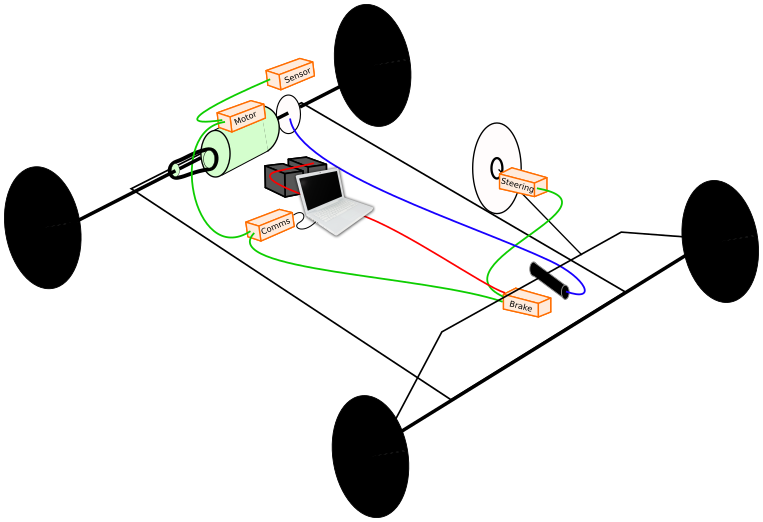
\includegraphics[width=\linewidth]{Images/layout}
    \caption{Locations of PCBs for go-kart}
    \label{locations}
  \end{figure}


  \subsection{Communications Network}
  Because the go-kart was required to be controlled by distributed hardware,
  some way of having the hardware communicate was required. To solve this
  problem, Local Interconnect Network (LIN Bus), Controller Area Network (CAN
  Bus), Universal Asynchronous Receiver/Transmitter (UART) and Serial
  Peripheral Interface Bus (SPI) were evaluated as viable options. Both LIN and
  CAN are serial communication buses designed for use in vehicle and automation
  systems, where UART and SPI are designed as simple serial communications.
  
  \begin{itemize}
    \item[LIN]{LIN is a single wire communications standard which supports
    speeds of up to 19.2kbit/s\cite{LIN}. It is a master slave design which
    supports up to sixteen slaves. The data frame on the LIN Bus is variable
    length of either 2, 4 or 8 bytes. There is no collision detection, however
    data checksumming and error detection is implemented in the standard.  LIN
    was designed in 1999 with further LIN standards released in 2002 and 2003.}

    \item[CAN]{CAN 2.0 is a master-master broadcast serial bus standard. It
    supports half-duplex data rates of up to 1Mbit/s. The CAN Bus uses a
    differential pair with the traffic encoded in non return to zero. Each
    packet is formatted with a header, including receivers address, followed by
    zero to eight bytes of data. Robert Bosch GmbH \cite{bosch} developed the
    standard in 1983, but now days the ISO11989 standard also describes CAN 2.0
    \cite{boschCAN, ISOCAN}.}

    \item[UART]{Using Universal Asynchronous Receiver/Transmitter was dropped
    as an idea rather early on. This is because it does not support the error
    correction that was needed for the project. Another area it was lacking is
    being expandable. A new UART would be required for each new node or
    device.}

    \item[SPI]{For much the same reasons UART was not used for our central
    communications bus, Serial Peripheral Interface Bus was also not
    appropriate.} 

  \end{itemize}

  It was decided to that using a CAN Bus would be the best option. Some major
  factors that influenced this choice were; the CAN standard had better
  documentation, later work can add more nodes into the network, hardware level
  collision and error detection and CAN controller supported by Atmel SAM7
  series micro controller. Atmel also provided a CAN transceiver
  IC\cite{ata666}, however this could have been replaced by a IC made by Texas
  Instruments\cite{ti-can-trans}.

  Although both UART and SPI were not used for the system bus, both can be used
  for local sensors, or other expansion modules.

  \subsection{Micro Controller}
  The main requirements of the micro controller are that it supports both a CAN
  controller and hardware USB. Also because previous projects had used either
  the Atmel ATMega or the Atmel AT91SAM7 micro controllers, we had preference
  of using these rather than learning a new architecture and data sheet format.

  \subsection{Motor Drivers}
  To drive the actuators for the steering and brake we decided to use a motor
  driver IC. By basing our motor driver circuit specification on the current
  draw of the steering motor, then reused the same design for the brake linear
  actuator. This was done both to save time in the hardware design, but also
  time in software later on\cite{Looman_2011}. The motor drives were placed on their own small PCB
  to save space on the main PCB and also provide more opportunity for heat
  dissipation if this were to become a problem. 

  The motor driver that was used is the DRV8432 made by Texas
  Instruments\cite{ti-motor-driver}. It is a dual full bridge PWM motor driver.
  It has a split logic and driving voltage, so it is driven directly from the
  batteries, but the control logic is at 3.3V. It has a peak voltage of 50V and
  a maximum current of 12A which is more than we need for either of the
  actuators. Figure \ref{motorPCB} shows one of the two motor driver boards with
  a heat sink covering the motor driver IC.

   \begin{figure}[h]
     \centering
     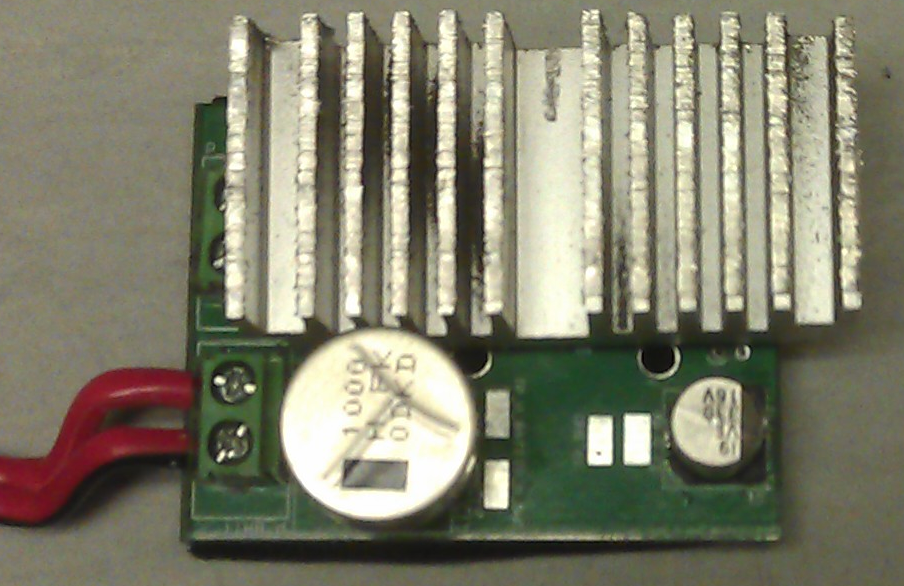
\includegraphics[width=.9\linewidth]{Images/motorPCB.png}
     \caption{Motor driver board for driving actuators}
     \label{motorPCB}
   \end{figure}


  \subsection{Expansion IO}
  To allow the hardware to be expandable, two 3.3V UARTs, one 3.3V SPI and
  one 5V logic SPI are been exposed on each PCB. Each serial port has it's own
  PicoBlade connector\cite{PicoBlade} as well as all the power supplies are
  exposed via another connector. All the serial port pins can also be set to be
  GPIO to allow them to be used for other purposes too.

  The 5V logic SPI is enabled via the use of a logic level shifter chip
  the MAX3001E made by Maxim \cite{MAX3001E}. To complement the 5V spi, a 5V
  external ADC is also on the boards. This was placed on the boards for the
  purpose of replacing the student board, but can be used for other analogue
  input too.

  \subsection{Encoder Reading}
  Because getting both speed and directions from an encoder signal in software
  is quite tricky, a quadrature clock converter was used. This takes in the
  encoder pulses and out puts a single pulse and which direction it is rotating
  in. Which allows a simple counter and incrementing or de-incrementing it to
  keep the actuators position.

  \subsection{Debugging}
  To make debugging easier, epically in the early stages of development, a two
  digit seven segment display and 4 push buttons are placed on each PCB. The
  display is driven by a display driver. This display driver takes a four bit
  number in parallel and converts it into the segment array lines. It is
  multiplexed with the second segment so by switching between the displays
  faster than 20Hz allows both digits to be used.

  \subsection{On Board Power}
  On each board there is four different voltage five levels. There is the
  battery voltage, which is only used by the voltage regulators, 3.3V, 5V, 12V
  and ground. Because we used a 4 layer PCB design, excluding the battery
  voltage, each of the voltage levels were spread across a whole plane on the
  PCB allowing better coupling between them and ground.

    \subsubsection{3.3 Volts}
    This was used by most of the logic components including the SAM7 micro
    controller. As less than 300mA was required and having a smooth, non-rippled,
    voltage would ensure the micro controller ran well, a linear voltage
    regulator was used.

    \subsubsection{5 Volts}
    The main reason for having 5 volts on the boards was to allow a 3.3V to 5V
    logic translator to be used. This level shifter is required by the student
    board in the power electronics. A linear voltage regulator was used here
    also.

    \subsubsection{12 Volts}
    Both the inductance sensor used for speed detection and the motor driver
    required 12 volts, which both of these applications use less than 150mA so a
    TPS7A4901 linear voltage regulator was used\cite{TPS7A4901}.

